\subsection{Partes} \label{subsec:partes}
Información de las piezas del robot. 

\textbf{1-Parametros del motor NEMA 17}
\begin{figure} [h]
	\centering
	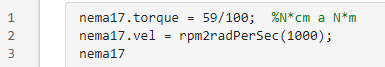
\includegraphics[width=0.7\linewidth]{img/calculomotores1}
	\caption{Parametros del motor NEMA 17}
	\label{fig:calculomotores1}
\end{figure}


-59/100 convierte el torque de 59 N·cm a 0.59 N·m.

-Se usa rpm2radPerSec() para convertir 1000 rpm a radianes por segundo.

-Se imprime el resultado.


\textbf{2-Parametros del motor NEMA 23}
\begin{figure} [h]
	\centering
	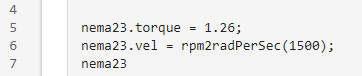
\includegraphics[width=0.7\linewidth]{img/calculomotores2}
	\caption{Parametros del motor NEMA 23}
	\label{fig:calculomotores2}
\end{figure}


-Se inicializa el motor NEMA 23 con su torque y velocidad, ya en unidades estándar del SI.

\newpage
\textbf{3-Parametros del servo}
\begin{figure} [h]
	\centering
	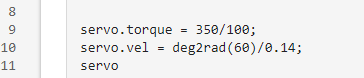
\includegraphics[width=0.7\linewidth]{img/calculomotores3}
	\caption{Parametros del servo}
	\label{fig:calculomotores3}
\end{figure}

-Calcula cuántos rad/s representa girar 60° en 0.14 s.


\textbf{4-Articulación 1: motor NEMA 17 con polea}

\begin{figure} [h]
	\centering
	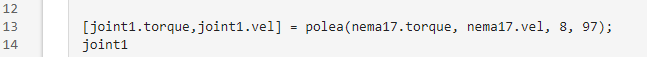
\includegraphics[width=0.7\linewidth]{img/calculomotores4}
	\caption{motor NEMA 17 con polea}
	\label{fig:calculomotores4}
\end{figure}

-Se usa una transmisión por poleas con una entrada de 8 mm y salida de 97 mm.

-Aumenta el torque y reduce la velocidad proporcionalmente.


\textbf{5-Articulación 2: NEMA 23 + polea + engranaje}


\begin{figure} [h]
	\centering
	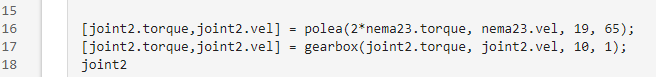
\includegraphics[width=0.7\linewidth]{img/calculomotores5}
	\caption{NEMA 23 + polea + engranaje}
	\label{fig:calculomotores5}
\end{figure}


-Se suman los torques de dos motores NEMA 23.

-Pasa por una polea (19 mm entrada, 65 mm salida) y una caja reductora (relación 10:1).

-El torque aumenta en ambas etapas, la velocidad disminuye.

\newpage
\textbf{6-Articulación 3: NEMA 17 + polea + engranaje}

\begin{figure} [h]
	\centering
	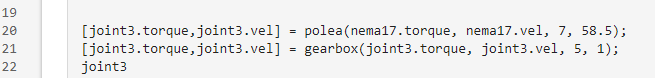
\includegraphics[width=0.7\linewidth]{img/calculomotores6}
	\caption{NEMA 17 + polea + engranaje}
	\label{fig:calculomotores6}
\end{figure}


-Primero, el torque y la velocidad del motor NEMA 17 pasan por una polea con un diámetro de entrada de 7 mm y salida de 58.5 mm.

-Esto incrementa el torque y reduce la velocidad angular en proporción al cociente 58.5/7

-Después, los valores resultantes pasan por una caja reductora con una relación de 5:1.

-Nuevamente, el torque se multiplica por 5, y la velocidad se divide por 5.

-Resultado: aumento significativo del torque y gran reducción de velocidad, ideal para tareas de fuerza con baja velocidad.


\textbf{7-Articulación 4: Motor NEMA 17 con una sola polea}

\begin{figure} [h]
	\centering
	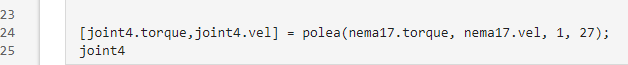
\includegraphics[width=0.7\linewidth]{img/calculomotores7}
	\caption{Motor NEMA 17 con una sola polea}
	\label{fig:calculomotores7}
\end{figure}


-Este caso modela una polea simple con una gran relación 27/1, es decir:

Aumenta 27 veces el torque.

Disminuye la velocidad 27 veces.

-Útil para articulaciones que requieren alta fuerza con muy poca velocidad, como agarres o soportes


\textbf{8-Articulación 5: Servo directamente}


\begin{figure} [h]
	\centering
	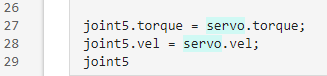
\includegraphics[width=0.7\linewidth]{img/calculomotores8}
	\caption{Servo directamente}
	\label{fig:calculomotores8}
\end{figure}


-No se aplica ni polea ni engranaje.

-Se asignan directamente el torque y la velocidad angular del servo motor a la articulación 5.

-Esto representa un accionamiento directo, normalmente en aplicaciones donde ya se ha diseñado el servo para cumplir con los requerimientos mecánicos de torque y velocidad.


%\subsubsection{Motores} \label{subsubsec:motores}
%Explicarán cuál es el motor que usaron, harán referencia a la hoja de datos, así como las transmisiones (por ejemplo, las de las pinzas) o reductores de velocidad a los que están acoplados. Deben de poner también información como: masa, fuerza o torque máximo, razón de reducción (por ejemplo, 10/1) y la velocidad máxima.
%%\subsubsection{Eslabones} \label{subsubsec:eslabones}
%Pondrán la masa, inercia, longitud y material de cada eslabón.